\section{Hierarchisches Modell für korrelierte Felder}\label{k4.2.hiera}
\sectionauthor{Natalie Teplitska, Clemens Ljungh, Constantin Burmeister}
Das Projekt \emph{Hierarchisches Modell für korrelierte Felder} beschäftigte sich mit der Bestimmung eines Priors $P(s)$ für korrelierte Felder. Diese Aufgabe wurde mit den Hilfsmitteln der Python-Bibliothek \emph{NIFTy8} gelöst.

Ziel eines bildgebenden Verfahrens ist die Ermittlung der quantity of interest $s$. Dies kann bei der Radioastronomie die Helligkeit des Himmels oder bei der CT die Dichte des untersuchten Objektes sein. Da weder Helligkeit noch Dichte negativ sein kann, setzen wir $s \geq 0$ voraus. Damit lässt sich eine Normalverteilung für $P(s)$ bereits ausschließen, da eine solche in ganz $\mathbb{R}$ definiert wäre. Außerdem wird angenommen, dass die einzelnen Bildpunkte miteinander korreliert sind, also voneinander abhängen. Ist zum Beispiel ein Pixel schwarz, so ist es unwahrscheinlich, dass sich in direkter Nähe dazu weiße Pixel befinden. In unserem Fall gilt, dass die Abhängigkeit zunimmt, je kleiner dar Abstand zwischen zwei Pixeln ist. Daraus ergibt sich eine schwierig zu verarbeitende Kovarianzmatrix, die die Korrelation der Pixel zueinander codiert.

Die Annahme, die Korrelation zwischen Pixeln sei normalverteilt, stellt häufig eine gute Näherung dar. In unserem Fall ist es jedoch das Ziel, ein hierarchisches Modell zu erzeugen, um einen Prior mit besseren Näherungen zu verwenden.

Dazu verwenden wir als Zufallsvariable nicht mehr $s$, sondern $\xi$, welches mit $P(\xi) = \mathbb{G}(\xi, \mathds{1})$ standard-normalverteilt ist. Diese ist in jedem Freiheitsgrad mit Erwartungswert 0 und Varianz 1 normalverteilt.

Unsere Aufgabe bestand nun darin, eine Funktion $f$ so zu definieren und zu implementieren, sodass $P(f(\xi)) d \xi = P(s) ds$. Die Schwierigkeit liegt hierbei insbesondere in der oben erwähnten Komplexität der Kovarianzmatrix.

Die \emph{Cholesky-Zerlegung} \href{https://www.uni-muenster.de/AMM/num/Vorlesungen/Numerik1_WS06/loesungen06/Prog_cholesky.pdf}{uni-muenster.de}
stellt eine Möglichkeit dar, einen solchen Prior zu erzeugen, wobei nur eine Dreiecksmatrix mit halb so vielen Einträgen gespeichert werden muss. Dies geschieht, indem im übertragenen Sinn die Wurzel aus $S$ gezogen wird, sodass $S=A A^{\dagger}$. Auf diese Weise lässt sich eine Funktion definieren, die aus zufälligen Zahlen $\xi$ den Prior berechnet: $s = f(\xi) = A \cdot \xi$. Allerdings ist der Speicherverbrauch der Dreiecksmatrix für $\mathcal{O}(100 000)$ Datenpunkte immer noch enorm.

Ein alternatives Verfahren stellt das \emph{Wiener-Chintchin-Theorem} dar. Hier wird die Annahme über die Kovarianz zwischen Pixeln nur über deren Entfernung, nicht jedoch über die Position getroffen. Dabei gilt
\begin{eqnarray}
S= \mathcal{F}^{\dagger} diag(p(|k|)) \mathcal{F}
\end{eqnarray}
Mit $diag(p(|k|))$ wird nur die Diagonale einer Diagonalmatrix gespeichert, welche durch eine Hartley-Transformation\footnote{Variante der Fourier-Transformation, welche Real- und Imaginärteil im reellen Raum verrechnet} erzeugt wird. Sie arbeitet mit der power function $p(|k|)$, die die Kovarianz kodiert. Dabei repräsentiert der Betrag von $k$ die Entfernung zwischen einzelnen Pixeln. Dieses Verfahren ist effizienter, da die Menge der Zahlen, welche in der Diagonalmatrix gespeichert werden muss, linear skaliert und auch die Hartley-Transformation keine vollständige Matrix benötigt, um korrekt ausgeführt zu werden.

Bisher haben wir mit einer vorgegebenen Kovarianz $S$ gearbeitet. Um aus Daten lernen zu können, dürfen wir uns allerdings nicht auf einen bestimmten Prior festlegen. Die Berechnung des Posteriors gestaltet sich wesentlich einfacher, wenn die power function - mit einigen vorausgesetzten Annahmen - über eine Menge von Parametern definiert wird. Diese können jeweils mit Bayes \cref{k4.2.bayes} immer weiter angepasst werden. Für unseren Fall arbeiteten wir mit drei Parametern %ref Bild
.
\begin{figure}[h] 
    \centering
    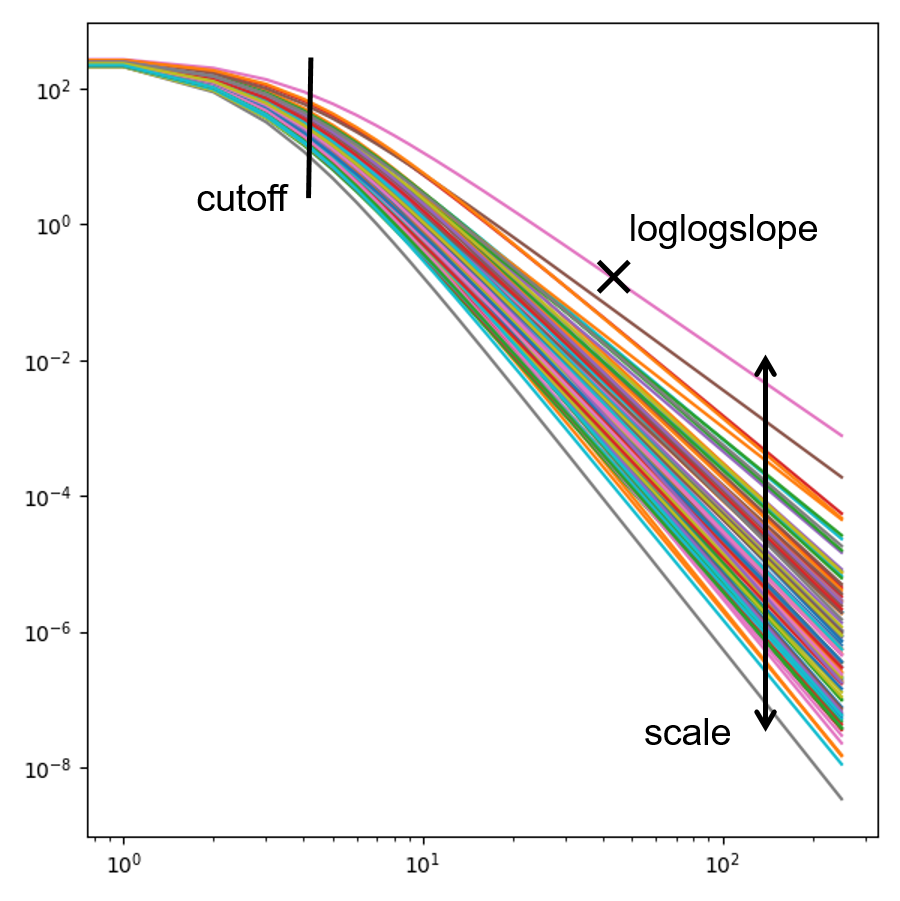
\includegraphics{k4.2/power_function_bearbeitet.png}
    \caption{100 beispielhafte power functions und ihre Parameter}
\end{figure}
\begin{itemize}
    \item Der Parameter \emph{scale} steht für die Standardabweichung der power function und beschreibt somit, wie stark sie variieren kann.
    \item Wir gehen von einer Funktion aus, die rechts von einem bestimmten Punkt eine Form annimmt, welche einem power-law folgt. Diesen Punkt bezeichnet man als \emph{cutoff}.
    \item Schließlich bezeichnet \emph{loglogslope} die Steigung der Funktion in dem Intervall nach dem cutoff.
\end{itemize}
Alle drei Parameter werden über je zwei Zahlenwerte definiert: den Mittelwert der Erwartungen und seine vermutete Varianz. Im Grunde genommen arbeiten wir also mit sechs Zahlenwerten, die unter Einbezug von Daten immer weiter angepasst werden können.

Damit haben wir es geschafft, einen Prior mittels Zufallszahlen zu generieren, der ein Lernen aus Daten mit kleinstmöglichem Rechen- und Speicheraufwand ermöglicht.
